\documentclass[11pt, a4paper]{report}
\usepackage[utf8]{inputenc}
\usepackage[portuguese]{babel}
\usepackage{color}
\usepackage{graphicx}
\usepackage{ulem}
\usepackage[bottom]{footmisc}
\usepackage[utf8]{inputenc}
\title{A Série de TV Guerra dos Tronos}
\author{Nome do autor}
\date{}
\begin{document}

\maketitle
\chapter{Introdução}
\section{Sobre a série}
\label{sec:sobre}
A {\Huge Guerra dos Tronos}\footnote{Este é o nome de uma marca registada.} é uma super produç\~ao televisiva da HBO, baseada na saga literária de George R.R. Martin, é uma série que {\tiny redefine os parâmetros do que é possível fazer em televis\~ao}.

\vspace{1cm}

{\centering \textit{Uma narrativa épica que {\Large atravessa mundos imaginários} e personagens a perder de vista.} \footnote{Texto retirado de http://tv.sapo.pt/series/a-guerra-dos-tronos.}.\par}

\vspace{1cm}

\begin{verbatim}
UPS! Este texto não deveria estar aqui / § " º % $ & ^ ~
\end{verbatim}

\section{Elenco}
\label{sec:elen}
A secç\~ao~\ref{sec:sobre} falou-nos sobre a série e agora na secç\~ao~\ref{sec:elen} vamos falar sobe o elenco. A tabela~\ref{tab:tab} mostra-nos as personagens principais.

\begin{table}[]
\centering
\begin{tabular}{|l|c|r|}
\hline
\textbf{Ator/atriz} & \textbf{Personagem} & \textbf{Temporada} \\ \hline
Peter Dinklage      & Tyrion Lannister    & 1,2 e 3            \\ \hline
Emilia Clarke       & Daenerys Targaryen  & 1,2 e 3            \\ \hline
Richard Madden      & Robb Stark          & 1e 2               \\ \hline
\end{tabular}
\caption{Principais personagens da "Guerra dos Tronos" ao longo das várias temporadas.}
\label{tab:tab}
\end{table}

\begin{figure}
\centering
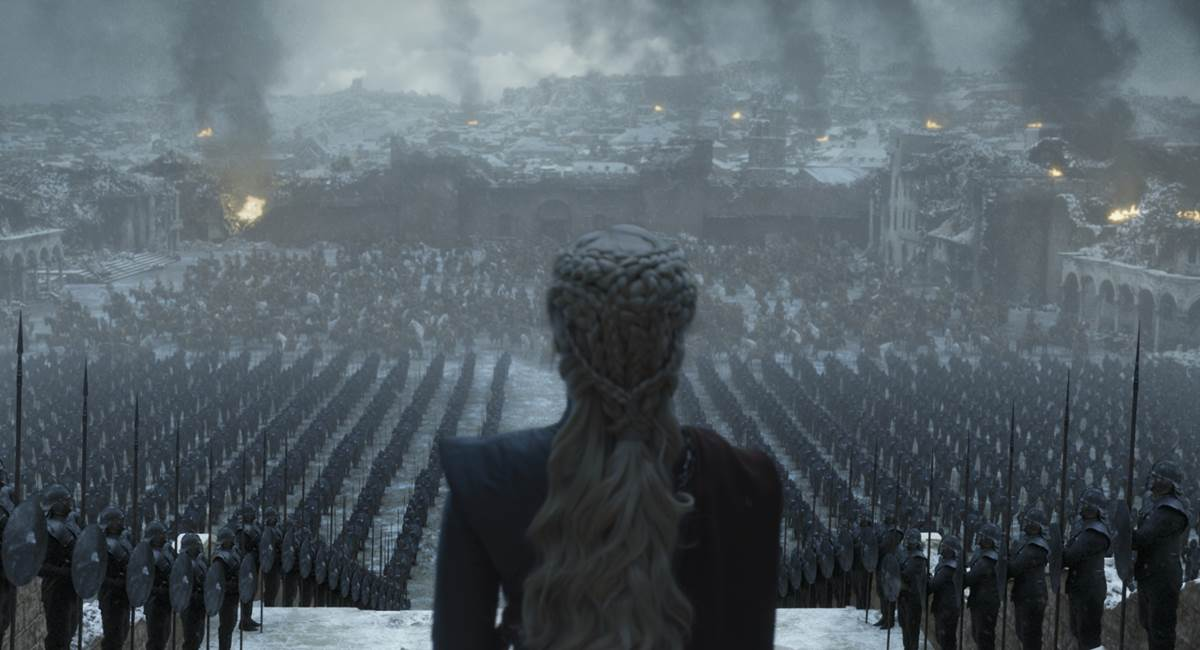
\includegraphics[scale=0.3]{got.jpg}
\end{figure}

\end{document}